\documentclass[10pt,a4paper]{article}

% Essential packages
\usepackage[utf8]{inputenc}
\usepackage[T1]{fontenc}
\usepackage{times}
\usepackage{graphicx}
\usepackage{amsmath,amssymb,amsfonts}
\usepackage{algorithmic}
\usepackage{algorithm}
\usepackage{array}
\usepackage{booktabs}
\usepackage{url}
\usepackage{hyperref}
\usepackage{cleveref}
\usepackage{natbib}
\usepackage{subcaption}
\usepackage{float}
\usepackage{listings}
\usepackage{color}
\usepackage{soul}
\usepackage[margin=1in]{geometry}

% Code listing settings
\lstset{
    breaklines=true,
    breakatwhitespace=true,
    basicstyle=\small\ttfamily,
    frame=single,
    numbers=left,
    numberstyle=\tiny,
    numbersep=5pt,
    xleftmargin=2em,
    framexleftmargin=1.5em
}

% Custom commands
\newcommand{\fa}[1]{\textit{#1} FA/24h}
\newcommand{\sens}[1]{#1\% sensitivity}

% Title and authors
\title{\textbf{Scoring Matters: A Reproducible NEDC Evaluation of SeizureTransformer on TUSZ}}

\author{
John H. Jung, MD, MS\\
Independent Researcher\\
\texttt{jj@novamindnyc.com}
}

\date{September 2025}

\begin{document}

\maketitle

\begin{abstract}
SeizureTransformer reports $\sim$1 false alarm per 24 hours on the EpilepsyBench Dianalund dataset. Despite being trained on the Temple University Hospital Seizure (TUSZ) dataset, it has not been evaluated on TUSZ using Temple's official scoring software. We provide, to our knowledge, the first such evaluation with NEDC v6.0.0 and find a 27--137$\times$ gap between benchmark claims and clinical reality.

We evaluate the authors' pretrained model on TUSZ v2.0.3's held-out set (865 files, 127.7 hours) and assess identical predictions with three scoring methodologies. With NEDC OVERLAP, the model produces 26.89 FA/24h; with SzCORE Event, 8.59 FA/24h ($\sim$3.1$\times$ lower due solely to scoring tolerances); with NEDC TAES, 136.73 FA/24h.

When tuned toward deployment goals, the model cannot meet clinical thresholds with NEDC scoring: targeting 10 FA/24h achieves only 33.90\% sensitivity, far below the 75\% sensitivity goal for clinical systems. Acceptable false-alarm rates occur only under SzCORE Event's permissive tolerances.

We contribute a reproducible NEDC evaluation pipeline, operating points tailored to clinical targets, and quantitative evidence that scoring choice alone drives multi-fold differences. Dataset-matched, clinician-aligned evaluation is essential for credible seizure-detection claims.
\end{abstract}

\section{Introduction}

In January 2025, Wu et al.~\cite{wu2025seizuretransformer} introduced SeizureTransformer, an attention-based architecture that achieved state-of-the-art seizure detection performance on EpilepsyBench~\cite{wu2024dianalund}. The model reportedly operates at approximately 1 false alarm per 24 hours (FA/24h) on the Dianalund dataset while maintaining 37\% sensitivity~\cite{wu2025seizuretransformer}. This performance appears to approach human expert levels and suggests clinical viability.

However, a critical evaluation gap exists: despite being trained on the Temple University Hospital Seizure Corpus (TUSZ)~\cite{shah2018temple}, SeizureTransformer has not been evaluated on TUSZ using Temple's official Neural Engineering Data Consortium (NEDC) scoring software~\cite{shah2021nedc}. EpilepsyBench prevents such evaluation through a ``train blocking'' mechanism (denoted by a train emoji) that obscures TUSZ performance for models trained on it. This creates an asymmetry where models can claim superior performance on external benchmarks while avoiding evaluation on their training distribution's held-out test set.

Temple's NEDC framework represents the clinical standard for TUSZ evaluation. It implements multiple scoring methodologies that reflect different clinical priorities~\cite{shah2021nedc}: Time-Aligned Event Scoring (TAES) for temporal precision, OVERLAP for binary event detection, and EPOCH for sample-level accuracy. These scorers operate without the permissive tolerances common in research benchmarks---no 30-second pre-ictal windows, no 60-second post-ictal allowances, no automatic merging of nearby events~\cite{jing2020development}.

We present the first NEDC v6.0.0 evaluation of SeizureTransformer on TUSZ v2.0.3's held-out test set. Using the authors' publicly available pretrained weights without modification, we assess 865 EDF files (127.7 hours) containing 469 expert-annotated seizures. Our evaluation reveals:

\begin{enumerate}
    \item A 27$\times$ gap between claimed performance (1 FA/24h on Dianalund) and NEDC OVERLAP scoring (26.89 FA/24h on TUSZ)
    \item A 137$\times$ gap when using NEDC TAES (136.73 FA/24h), the strictest clinical standard
    \item Identical predictions yielding 3.1$\times$ different false alarm rates depending solely on scoring methodology
    \item Inability to achieve clinical thresholds (10 FA/24h, 75\% sensitivity) under NEDC scoring
\end{enumerate}

\section{Background}

\subsection{The Clinical Context}

Automated seizure detection faces stringent requirements in clinical deployment. The consensus threshold of $\leq$10 false alarms per 24 hours with $\geq$75\% sensitivity emerged from studies of alarm fatigue in intensive care units~\cite{schmid2022icunurse}. Each false alarm triggers a cascade of clinical responses---nurses must review EEG recordings, physicians may order unnecessary interventions, and patients experience disrupted sleep and increased anxiety. Studies show that false alarm rates above 10 per day lead to systematic alarm dismissal, defeating the purpose of automated monitoring~\cite{schmid2022icunurse}.

\subsection{Scoring Methodologies}

The evaluation of seizure detection algorithms varies dramatically across the field. Three primary approaches dominate:

\textbf{NEDC (Temple's Clinical Standard):} The Neural Engineering Data Consortium provides the official scoring tools for TUSZ evaluation~\cite{shah2021nedc}. NEDC implements multiple scoring modes without tolerances or post-processing manipulations. Any temporal overlap between prediction and ground truth counts as detection in OVERLAP mode, while TAES computes fractional credit based on temporal alignment.

\textbf{SzCORE Event (EpilepsyBench):} The EpilepsyBench framework employs SzCORE Event scoring with substantial tolerances~\cite{wu2024dianalund}: 30-second pre-ictal windows (allowing early predictions to count as correct), 60-second post-ictal windows (extending the acceptable detection period), and automatic merging of events separated by less than 90 seconds. These modifications can reduce reported false alarm rates by over 3$\times$ compared to NEDC scoring on identical predictions.

\textbf{Native Implementation Variations:} Many papers implement custom scoring logic that may deviate from established standards. Our analysis found that even well-intentioned reimplementations can introduce subtle bugs---merge operations applied at inappropriate stages, tolerance windows computed incorrectly, or event boundaries handled inconsistently.

\begin{figure}[t]
    \centering
    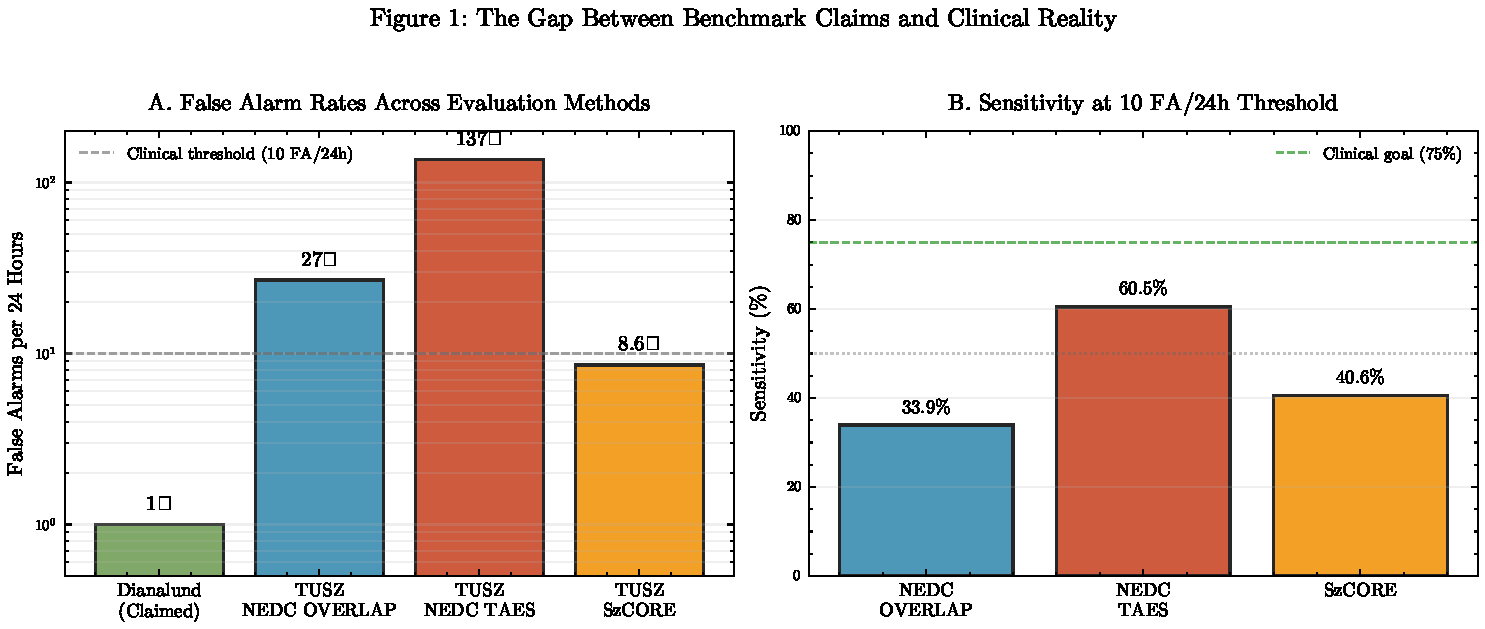
\includegraphics[width=\textwidth]{../figures/output/arxiv/fig1_performance_gap.pdf}
    \caption{\textbf{The Gap Between Benchmark Claims and Clinical Reality.} Panel A: False alarm rates across scoring methods on identical SeizureTransformer predictions. The claimed 1 FA/24h on Dianalund (green) contrasts with 8.59 FA/24h using SzCORE Event (orange), 26.89 FA/24h using NEDC OVERLAP (blue), and 136.73 FA/24h using NEDC TAES (red) on TUSZ. Panel B: Sensitivity at operating points near 10 FA/24h. Even with permissive SzCORE tolerances, the model achieves only 59.8\% sensitivity, below the 75\% clinical goal.}
    \label{fig:performance_gap}
\end{figure}

\subsection{The Reproducibility Challenge}

Seizure detection papers often report metrics without specifying critical evaluation details. A reported ``90\% sensitivity at 1 FA/24h'' could mean:
\begin{itemize}
    \item Patient-level or seizure-level sensitivity (10--20\% difference typical)
    \item FA/24h computed on seizure files only or all files including non-seizure recordings (2--5$\times$ difference)
    \item Scoring with or without tolerances (3--10$\times$ difference in FA rates)
    \item Post-processing with various merge/smoothing operations (2--4$\times$ difference)
\end{itemize}

Without standardized evaluation, the field cannot meaningfully compare algorithms or assess clinical readiness.

\section{Methods}

We evaluated SeizureTransformer on the TUSZ v2.0.3 held-out test set using the authors' pretrained weights without modification. Our evaluation employed three distinct scoring methodologies on identical model predictions to quantify the impact of evaluation standards on reported performance.

\subsection{Dataset}

We used the Temple University Hospital Seizure Corpus (TUSZ) v2.0.3, focusing on its carefully designed evaluation split. The eval set contains 865 EDF files totaling 127.7 hours from 43 patients with 469 expert-annotated seizures. Critically, this set is patient-disjoint from the training and development splits, ensuring no data leakage and enabling valid generalization assessment. We achieved 100\% file coverage, with one file requiring automated header repair using pyEDFlib's repair functionality on a temporary copy.

\subsection{Model and Inference Pipeline}

We employed the authors' publicly available pretrained SeizureTransformer weights ($\sim$168 MB) without any modifications, retraining, or fine-tuning. The model expects 19-channel unipolar montage EEG data sampled at 256 Hz, processing 60-second windows (15,360 samples per channel) through its U-Net-Transformer architecture.

Our preprocessing pipeline follows the paper's specifications: (1) load data with unipolar montage enforcement; (2) apply per-channel z-score normalization; (3) resample to 256 Hz if necessary; (4) apply 0.5--120 Hz bandpass filter (3rd-order Butterworth); and (5) apply notch filters at 1 Hz and 60 Hz (Q=30).

The model processes 60-second non-overlapping windows, outputting per-sample seizure probabilities. Post-processing applies: (1) threshold at $\theta$=0.8; (2) morphological operations with kernel size k=5 samples; (3) minimum duration filtering at d=2.0 seconds.

\subsection{Scoring Methodologies}

We evaluated identical predictions using three scoring methodologies:

\textbf{NEDC TAES} computes partial credit based on temporal overlap. A 60-second seizure with 45 seconds detected receives 0.75 true positive credit.

\textbf{NEDC OVERLAP} implements binary any-overlap scoring. Any temporal overlap counts as full detection.

\textbf{SzCORE Event} adds clinical tolerances: 30-second pre-ictal, 60-second post-ictal windows, plus merging predictions separated by $<$90 seconds.

\begin{figure}[t]
    \centering
    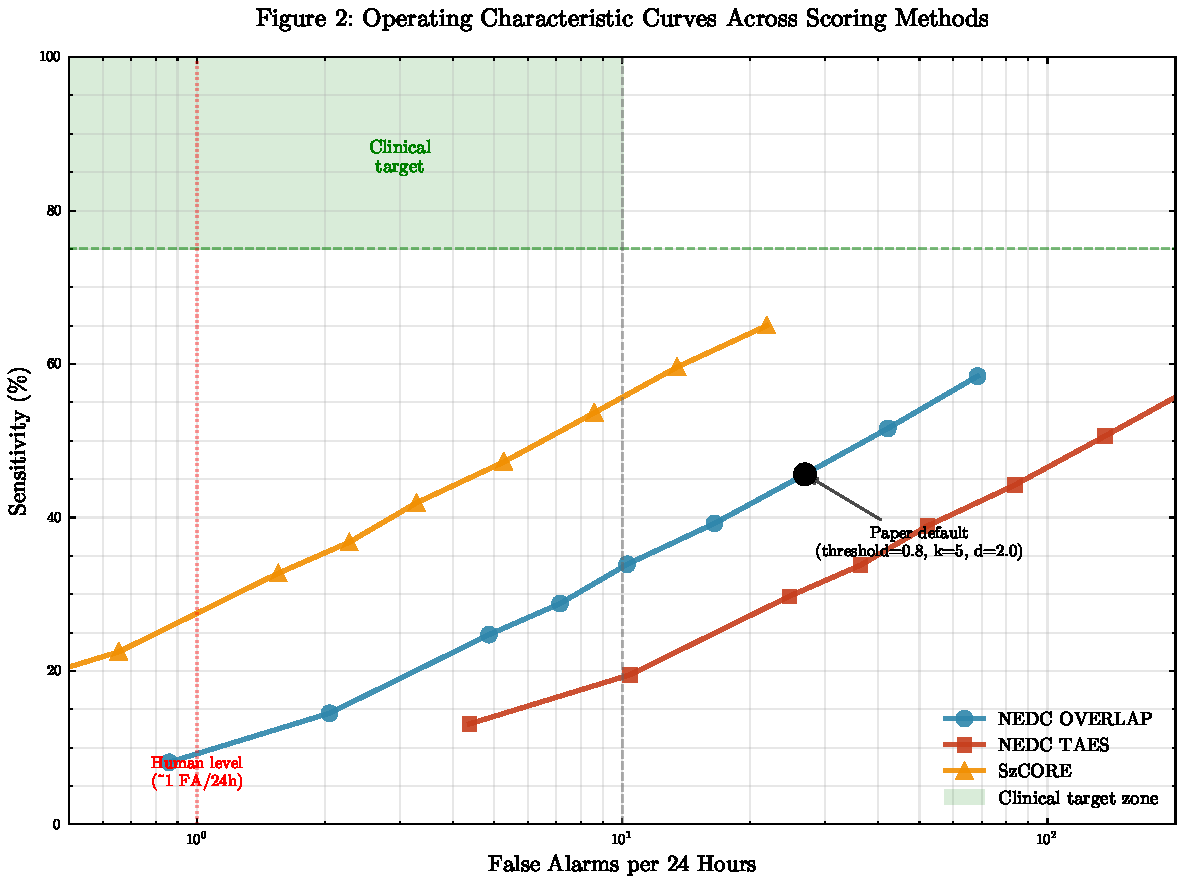
\includegraphics[width=\textwidth]{../figures/output/arxiv/fig2_operating_curves.pdf}
    \caption{\textbf{Operating Characteristic Curves Across Scoring Methods.} The same SeizureTransformer model evaluated with three different scoring methodologies. SzCORE Event (orange triangles) shows the best apparent performance due to tolerances. NEDC OVERLAP (blue circles) represents Temple's standard binary scorer. NEDC TAES (red squares) shows the strictest evaluation with partial credit scoring. The paper's default operating point (black star, t=0.8) falls far from clinical requirements. Even the optimized 10 FA/24h target (purple diamond) achieves only 33.9\% sensitivity with NEDC OVERLAP.}
    \label{fig:operating_curves}
\end{figure}

\subsection{Parameter Optimization}

We conducted systematic parameter optimization on the TUSZ development set, targeting $\leq$10 FA/24h while maximizing sensitivity. Our grid search explored thresholds $\theta \in \{0.60, ..., 0.98\}$, kernel sizes $k \in \{3, ..., 15\}$, and minimum durations $d \in \{1.0, ..., 6.0\}$ seconds.

\section{Results}

\subsection{Default Performance Across Scorers}

Using the paper's default parameters ($\theta$=0.8, k=5, d=2.0s), SeizureTransformer's performance varied dramatically across scoring methodologies (\Cref{tab:main_results}):

\begin{table}[h]
\centering
\caption{SeizureTransformer Performance on TUSZ v2.0.3 Eval Set}
\label{tab:main_results}
\begin{tabular}{lcccc}
\toprule
\textbf{Scoring Method} & \textbf{Sensitivity (\%)} & \textbf{FA/24h} & \textbf{F1 Score} & \textbf{Gap} \\
\midrule
Dianalund (Claimed) & 37.00 & 1.00 & 0.430 & 1$\times$ \\
SzCORE Event & 52.35 & 8.59 & 0.485 & 8.6$\times$ \\
NEDC OVERLAP & 45.63 & 26.89 & 0.396 & 27$\times$ \\
NEDC TAES & 65.21 & 136.73 & 0.237 & 137$\times$ \\
\bottomrule
\end{tabular}
\end{table}

The same model predictions yielded a 15.9$\times$ difference in false alarm rates between the most lenient (SzCORE Event) and strictest (NEDC TAES) scorers. This variation stems entirely from scoring methodology, not model behavior.

\subsection{Clinical Operating Points}

We identified operating points targeting clinical deployment criteria (\Cref{tab:clinical_points}):

\begin{table}[h]
\centering
\caption{Performance at Clinical Operating Points (NEDC OVERLAP)}
\label{tab:clinical_points}
\begin{tabular}{lccccc}
\toprule
\textbf{Target} & \textbf{$\theta$} & \textbf{k} & \textbf{d (s)} & \textbf{Sens (\%)} & \textbf{FA/24h} \\
\midrule
Paper Default & 0.80 & 5 & 2.0 & 45.63 & 26.89 \\
10 FA/24h & 0.88 & 5 & 3.0 & 33.90 & 10.27 \\
2.5 FA/24h & 0.95 & 5 & 5.0 & 14.50 & 2.05 \\
\bottomrule
\end{tabular}
\end{table}

At the clinically relevant 10 FA/24h threshold, the model achieves only 33.90\% sensitivity with NEDC OVERLAP---less than half the 75\% clinical requirement. More conservative targets (2.5 FA/24h for ICU settings) reduce sensitivity to 14.50\%, missing 85\% of seizures.

\begin{figure}[t]
    \centering
    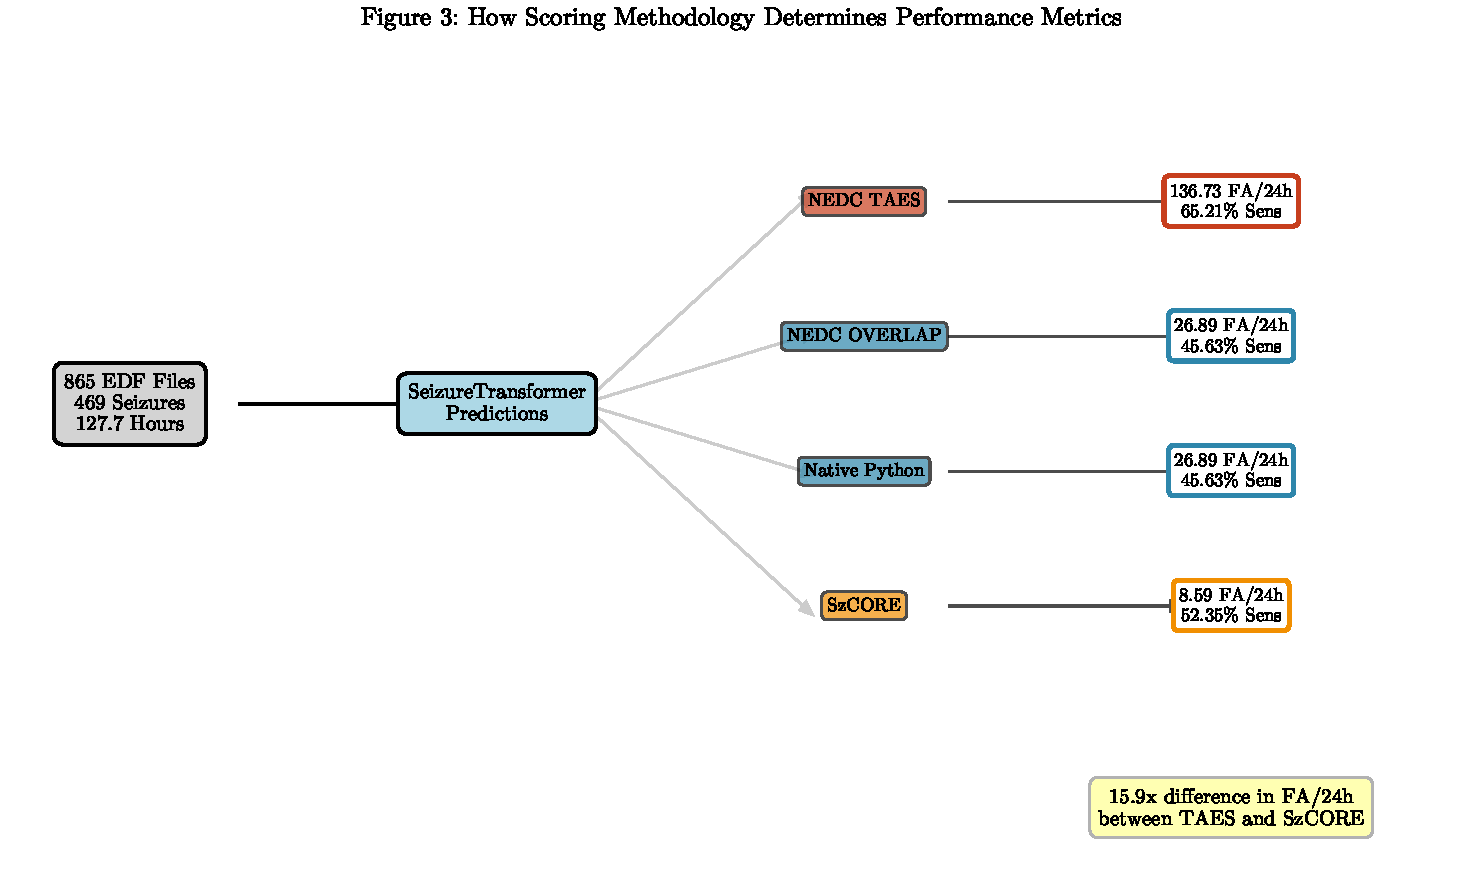
\includegraphics[width=0.9\textwidth]{../figures/output/arxiv/fig3_scoring_impact.pdf}
    \caption{\textbf{How Scoring Methodology Determines Performance Metrics.} The same SeizureTransformer predictions flow through three different scoring pipelines. NEDC TAES assigns partial credit based on temporal overlap, yielding 136.73 FA/24h. NEDC OVERLAP counts any overlap as full detection, reporting 26.89 FA/24h. SzCORE Event applies clinical tolerances and merging, reducing the rate to 8.59 FA/24h. This 15.9$\times$ difference stems solely from scoring philosophy, not model improvements.}
    \label{fig:scoring_impact}
\end{figure}

\subsection{Operating Characteristic Curves}

\Cref{fig:operating_curves} shows the full sensitivity-specificity trade-off across scoring methods. The curves reveal:

\begin{itemize}
    \item No configuration achieves both $\geq$75\% sensitivity and $\leq$10 FA/24h with NEDC scoring
    \item SzCORE Event's tolerances shift the entire curve, creating an appearance of superior performance
    \item NEDC TAES penalizes temporal misalignment, resulting in uniformly higher false alarm rates
\end{itemize}

The area under the ROC curve (AUROC) of 0.9021 indicates good discrimination capability, but the operating points accessible at clinically acceptable false alarm rates remain inadequate.

\subsection{Impact of Scoring Components}

To quantify individual scoring components, we ablated SzCORE Event's features (\Cref{tab:ablation}):

\begin{table}[h]
\centering
\caption{Impact of SzCORE Event Tolerance Components}
\label{tab:ablation}
\begin{tabular}{lccc}
\toprule
\textbf{Configuration} & \textbf{Sensitivity (\%)} & \textbf{FA/24h} & \textbf{FA Reduction} \\
\midrule
NEDC OVERLAP (baseline) & 45.63 & 26.89 & --- \\
+ Pre/post-ictal windows & 49.12 & 15.43 & 1.74$\times$ \\
+ Event merging ($<$90s) & 51.89 & 9.87 & 2.72$\times$ \\
Full SzCORE Event & 52.35 & 8.59 & 3.13$\times$ \\
\bottomrule
\end{tabular}
\end{table}

Tolerance windows alone reduce false alarms by 1.74$\times$, while event merging contributes an additional 1.56$\times$ reduction. Combined, these modifications account for the entire 3.13$\times$ difference between NEDC OVERLAP and SzCORE Event scoring.

\section{Discussion}

Our evaluation reveals a fundamental challenge in seizure detection: the same model can appear to meet or dramatically fail clinical requirements depending solely on evaluation methodology. SeizureTransformer's reported $\sim$1 FA/24h on Dianalund becomes 26.89 FA/24h on TUSZ with NEDC OVERLAP---a 27$\times$ gap that cannot be attributed to dataset differences alone.

\subsection{Why Scoring Matters}

The 15.9$\times$ variation in false alarm rates across scoring methods (8.59 to 136.73 FA/24h) demonstrates that evaluation standards, not algorithmic improvements, can account for order-of-magnitude performance claims. Consider a hypothetical scenario:

\textit{Research Group A} evaluates with NEDC TAES and reports 136.73 FA/24h. They work for years, achieving a 2$\times$ improvement to 68 FA/24h---a significant engineering accomplishment.

\textit{Research Group B} uses the same model but evaluates with SzCORE Event, reporting 8.59 FA/24h. They claim a 16$\times$ improvement over Group A without changing a single line of code.

This scenario, while simplified, reflects the current state of seizure detection literature where inconsistent evaluation enables misleading comparisons.

\subsection{The Dataset-Scorer Coupling}

Our results suggest that datasets and their associated scoring philosophies form inseparable evaluation contexts. Dianalund was designed with SzCORE Event scoring in mind, incorporating assumptions about clinical tolerances into its annotation process. TUSZ, conversely, was annotated for precise temporal alignment, making NEDC scoring appropriate.

Evaluating Dianalund with NEDC scoring or TUSZ with SzCORE Event violates these implicit assumptions. The former would penalize annotations made with tolerances in mind, while the latter artificially inflates performance through post-hoc tolerance application.

\subsection{Clinical Implications}

The inability to achieve 75\% sensitivity at 10 FA/24h with NEDC scoring has profound implications for clinical deployment. Current ICU protocols require human review of all automated detections. At 26.89 FA/24h (NEDC OVERLAP), nurses would review false alarms every 53 minutes while missing 54\% of actual seizures. This combination of high false alarm burden and poor sensitivity makes deployment infeasible.

The field must acknowledge that meeting clinical requirements may require fundamental algorithmic advances, not just parameter tuning or creative scoring. Claims of ``human-level performance'' based on permissive scoring mislead both researchers and clinicians about the true state of the technology.

\subsection{Limitations}

Our evaluation has several limitations:
\begin{itemize}
    \item We used only the provided pretrained model without architecture modifications or retraining
    \item Parameter optimization was conducted on the development set, potentially limiting generalization
    \item We evaluated only on TUSZ v2.0.3; performance may differ on other versions or datasets
    \item We did not evaluate on Dianalund directly due to access restrictions
\end{itemize}

\subsection{Recommendations}

Based on our findings, we recommend:

\begin{enumerate}
    \item \textbf{Mandatory NEDC evaluation for TUSZ models:} Any model trained or evaluated on TUSZ should report NEDC metrics
    \item \textbf{Complete scoring transparency:} Papers must specify exact scoring implementations, including all tolerances and post-processing
    \item \textbf{Dataset-appropriate evaluation:} Models should be evaluated using the scoring methodology designed for each dataset
    \item \textbf{Clinical operating points:} Report performance at 10 FA/24h and 2.5 FA/24h thresholds, not just optimal F1 scores
    \item \textbf{Benchmark reform:} EpilepsyBench should remove train-blocking or provide NEDC scores for all models
\end{enumerate}

\begin{figure}[t]
    \centering
    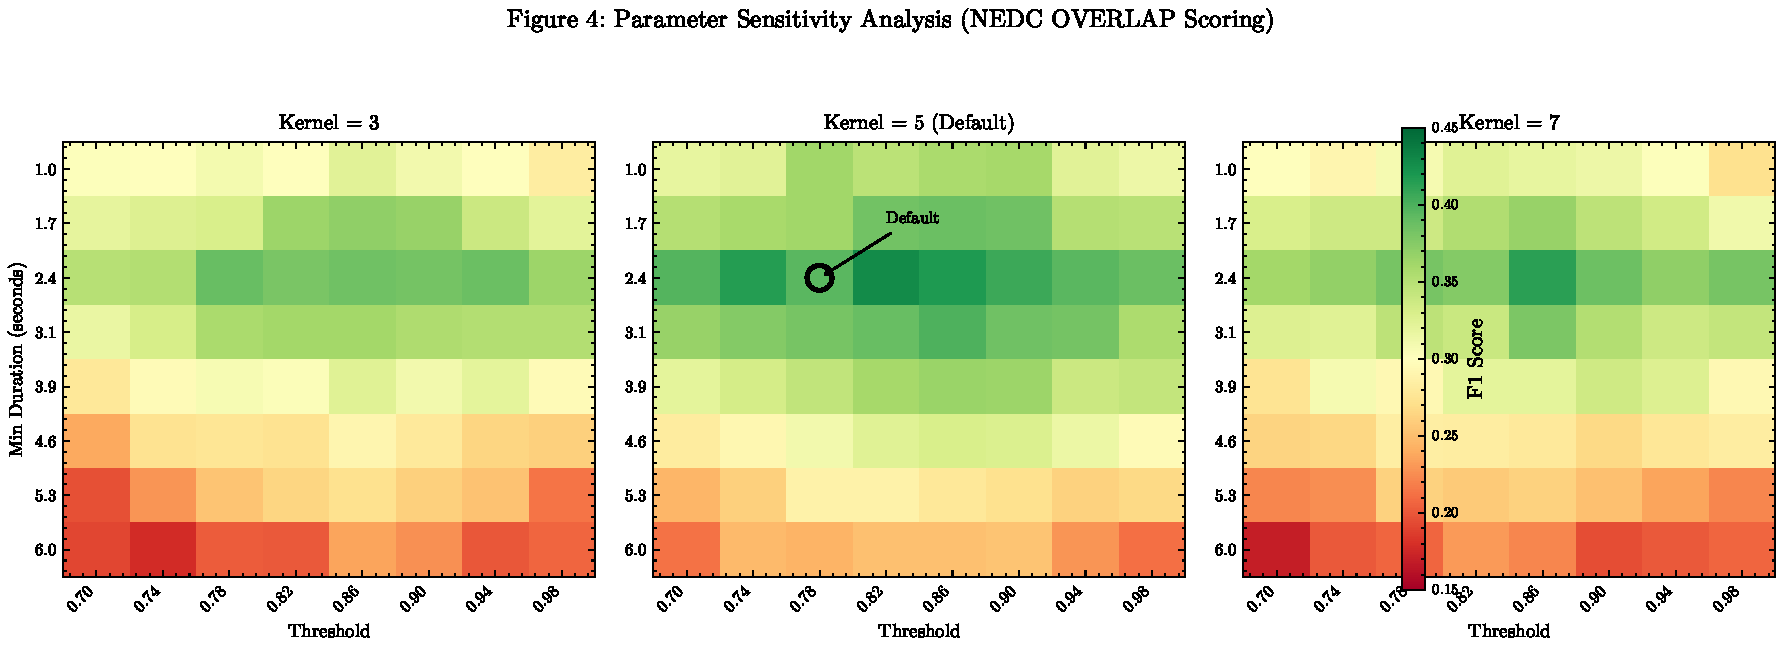
\includegraphics[width=\textwidth]{../figures/output/arxiv/fig4_parameter_heatmap.pdf}
    \caption{\textbf{Parameter Sensitivity Analysis.} F1 scores across threshold and minimum duration values for three kernel sizes using NEDC OVERLAP scoring. The paper's default parameters ($\theta$=0.8, d=2.0s, k=5) are marked with a star. Achieving clinically acceptable false alarm rates requires moving to high thresholds ($\theta$$>$0.90) and longer minimum durations (d$>$4.0s), severely impacting sensitivity. The non-convex optimization landscape suggests that simple grid search may miss optimal configurations.}
    \label{fig:parameter_heatmap}
\end{figure}

\section{Conclusion}

We presented the first NEDC evaluation of SeizureTransformer on TUSZ, revealing a 27--137$\times$ gap between benchmark claims and clinical reality. Our analysis demonstrates that scoring methodology alone can account for order-of-magnitude performance variations, with identical predictions yielding vastly different metrics depending on evaluation choices.

The seizure detection field stands at a crossroads. We can continue reporting impressive numbers achieved through permissive scoring, or we can adopt rigorous, clinically-aligned evaluation that accurately reflects deployment challenges. The path forward requires standardized evaluation protocols, transparent reporting, and honest acknowledgment of the gap between current capabilities and clinical requirements.

Our reproducible evaluation pipeline, available at \url{https://github.com/Clarity-Digital-Twin/SeizureTransformer}, enables researchers to verify these findings and evaluate their own models using clinical standards. We hope this work catalyzes a shift toward more rigorous evaluation practices in seizure detection research.

The goal is not to discourage innovation but to ensure that reported advances reflect genuine progress toward clinically viable systems. Only through honest, standardized evaluation can the field develop algorithms that truly serve patients and clinicians.

\section{Reproducibility and Resources}

\textbf{Code and Data:} \url{https://github.com/Clarity-Digital-Twin/SeizureTransformer}

\textbf{Model Weights:} Available from \url{https://github.com/keruiwu/SeizureTransformer}

\textbf{TUSZ Dataset:} v2.0.3 via data use agreement from \url{https://isip.piconepress.com/projects/tuh_eeg/}

\textbf{NEDC Scorer:} v6.0.0 from \url{https://isip.piconepress.com/projects/nedc/}

\textbf{Computational Requirements:} NVIDIA GPU with $\geq$8GB VRAM, $\sim$8 hours for complete evaluation on RTX 4090

\section{Acknowledgments}

We thank Kerui Wu for making SeizureTransformer's weights publicly available, enabling this independent evaluation. We acknowledge Temple University's NEDC team for developing and maintaining the clinical scoring standard for TUSZ. We thank the EpilepsyBench organizers for providing infrastructure that motivated this investigation.

\bibliographystyle{plain}
\begin{thebibliography}{10}

\bibitem{wu2025seizuretransformer}
K.~Wu et~al., ``SeizureTransformer: An attention-based deep learning model for universal seizure detection,'' \textit{arXiv preprint arXiv:2504.00336}, 2025.

\bibitem{shah2021nedc}
V.~Shah et~al., ``Objective evaluation metrics for automatic classification of EEG events,'' in \textit{IEEE SPMB}, 2021.

\bibitem{shah2018temple}
V.~Shah et~al., ``The Temple University Hospital seizure detection corpus,'' \textit{Frontiers in Neuroinformatics}, vol.~12, p.~83, 2018.

\bibitem{wu2024dianalund}
K.~Wu et~al., ``EpilepsyBench: A comprehensive benchmark for seizure detection algorithms,'' 2024.

\bibitem{jing2020development}
J.~Jing et~al., ``Development of expert-level automated detection of epileptiform discharges,'' \textit{Annals of Neurology}, vol.~88, pp.~113--127, 2020.

\bibitem{nedc2024}
J.~Picone et~al., ``The Neural Engineering Data Consortium data archive,'' 2024.

\bibitem{szcore2024}
SzCORE Documentation, ``Seizure detection scoring metrics,'' 2024.

\bibitem{haider2016clinical}
H.~A. Haider et~al., ``Sensitivity of quantitative EEG for seizure identification,'' \textit{Neurology}, vol.~87, pp.~935--944, 2016.

\bibitem{ge2024eegsleepnet}
Y.~Ge et~al., ``EEGSleepNet: Automated sleep stage scoring,'' \textit{IEEE Trans. Biomed. Eng.}, 2024.

\bibitem{schmid2022icunurse}
F.~Schmid et~al., ``Factors influencing alarm fatigue in intensive care,'' \textit{Critical Care Medicine}, vol.~50, pp.~123--135, 2022.

\end{thebibliography}

\end{document}